\documentclass[a4paper,11pt]{article}
\usepackage[utf8]{inputenc}
\usepackage[T1]{fontenc}
\usepackage{listings,color}
\usepackage{url}
\usepackage{amssymb}
\usepackage{amsmath}
\usepackage{color}
\usepackage{colortbl}
\usepackage{tabularx}
\usepackage{tikz}
\usepackage{float}
\usepackage{verbatim}
\usepackage{listings}
\usepackage[ngerman]{babel}

\usepackage{colortbl}
\usepackage{wrapfig}

\pagestyle{empty}
\setlength{\parindent}{0mm}

\newenvironment{mylist}{ \nopagebreak\begin{list}%
                           {(i)}%
                           {\topsep0cm \parsep0cm \partopsep0cm \itemsep0cm} }%
                       { \end{list} }

\definecolor{hellgrau}{cmyk}{0, 0, 0, 0.117}

\begin{document}

\lstset{language=bash, basicstyle=\ttfamily\tiny, backgroundcolor=\color{hellgrau}}

%\def\loesung
\textsc{Hochschule Fulda}{\small\hfill Einführung in Internetdienste}\\
{\small Fachbereich Angewandte Informatik{\small\hfill SS 11}\\
Dipl.-Inf. (HS) Ronny Trommer}\\

\begin{center}
{\Large\textbf{Lab Manual}}\\

\medskip
\end{center}

\smallskip

\newcommand{\half}{{\scriptstyle\frac{1}{2}}}
\newcolumntype{G}{>{\columncolor[gray]{0.9}}r}

\newcommand{\setK}{\mathbbm{K}}
\newcommand{\setR}{\mathbbm{R}}
\newcommand{\setZ}{\mathbbm{Z}}
\tableofcontents

\pagebreak

\section{Lab Dokumentation}
Der Versuchsaufbau wird im TK-Labor C106 durchgeführt. Für den Aufbau sind die
folgenden IP-Adressen vorgesehen:

\begin{tabular}[t]{l l l l l}
\hline
Netz-ID & Router & Srv1 & Srv2 & Domain \\
\hline
\textcolor{red}{192.168.1.0} & 192.168.1.1 & 192.168.1.2 & 192.168.1.3 &
beta.tklabor.site \\ 
\textcolor{red}{192.168.1.16} & 192.168.1.17 & 192.168.1.18 & 192.168.1.19 &
antares.tklabor.site
\\
\textcolor{red}{192.168.1.32} & 192.168.1.33 & 192.168.1.34 & 192.168.1.35 &
orion.tklabor.site \\
\textcolor{red}{192.168.1.48} & 192.168.1.49 & 192.168.1.50 & 192.168.1.51 &
vogsphere.tklabor.site \\
\hline
\textcolor{red}{192.168.1.64} & 192.168.1.65 & 192.168.1.66 & 192.168.1.67 &
frogstar.tklabor.site \\
\textcolor{red}{192.168.1.80} & 192.168.1.81 & 192.168.1.82 & 192.168.1.83 &
epun.tklabor.site \\
\textcolor{red}{192.168.1.96} & 192.168.1.97 & 192.168.1.98 & 192.168.1.99 &
earth.tklabor.site \\
\textcolor{red}{192.168.1.112} & 192.168.1.113 & 192.168.1.114 & 192.168.1.115 &
earth2.tklabor.site \\
\hline
\textcolor{red}{192.168.1.128} & 192.168.1.129 & 192.168.1.130 & 192.168.1.131 &
fallia.tklabor.site \\
\textcolor{red}{192.168.1.144} & 192.168.1.145 & 192.168.1.146 & 192.168.1.147 &
magrathea.tklabor.site \\
\textcolor{red}{192.168.1.160} & 192.168.1.161 & 192.168.1.162 & 192.168.1.163 &
lamuella.tklabor.site \\
\textcolor{red}{192.168.1.176} & 192.168.1.177 & 192.168.1.178 & 192.168.1.179 &
kria.tklabor.site \\
\hline
\textcolor{red}{192.168.1.192} & 192.168.1.193 & 192.168.1.194 & 192.168.1.195 &
zarss.tklabor.site \\
\textcolor{red}{192.168.1.208} & 192.168.1.209 & 192.168.1.210 & 192.168.1.211 &
rupert.tklabor.site \\
\textcolor{red}{192.168.1.224} & 192.168.1.225 & 192.168.1.226 & 192.168.1.227 &
eadrax.tklabor.site \\
\textcolor{red}{192.168.1.240} & 192.168.1.241 & 192.168.1.242 & 192.168.1.243 &
thesun.tklabor.site \\
\hline
\end{tabular}
\newline
\newline
Die entsprechenden Adressbereiche werden für die Gruppen wie folgt aufgeteilt:
\begin{figure}[H]
\begin{center}
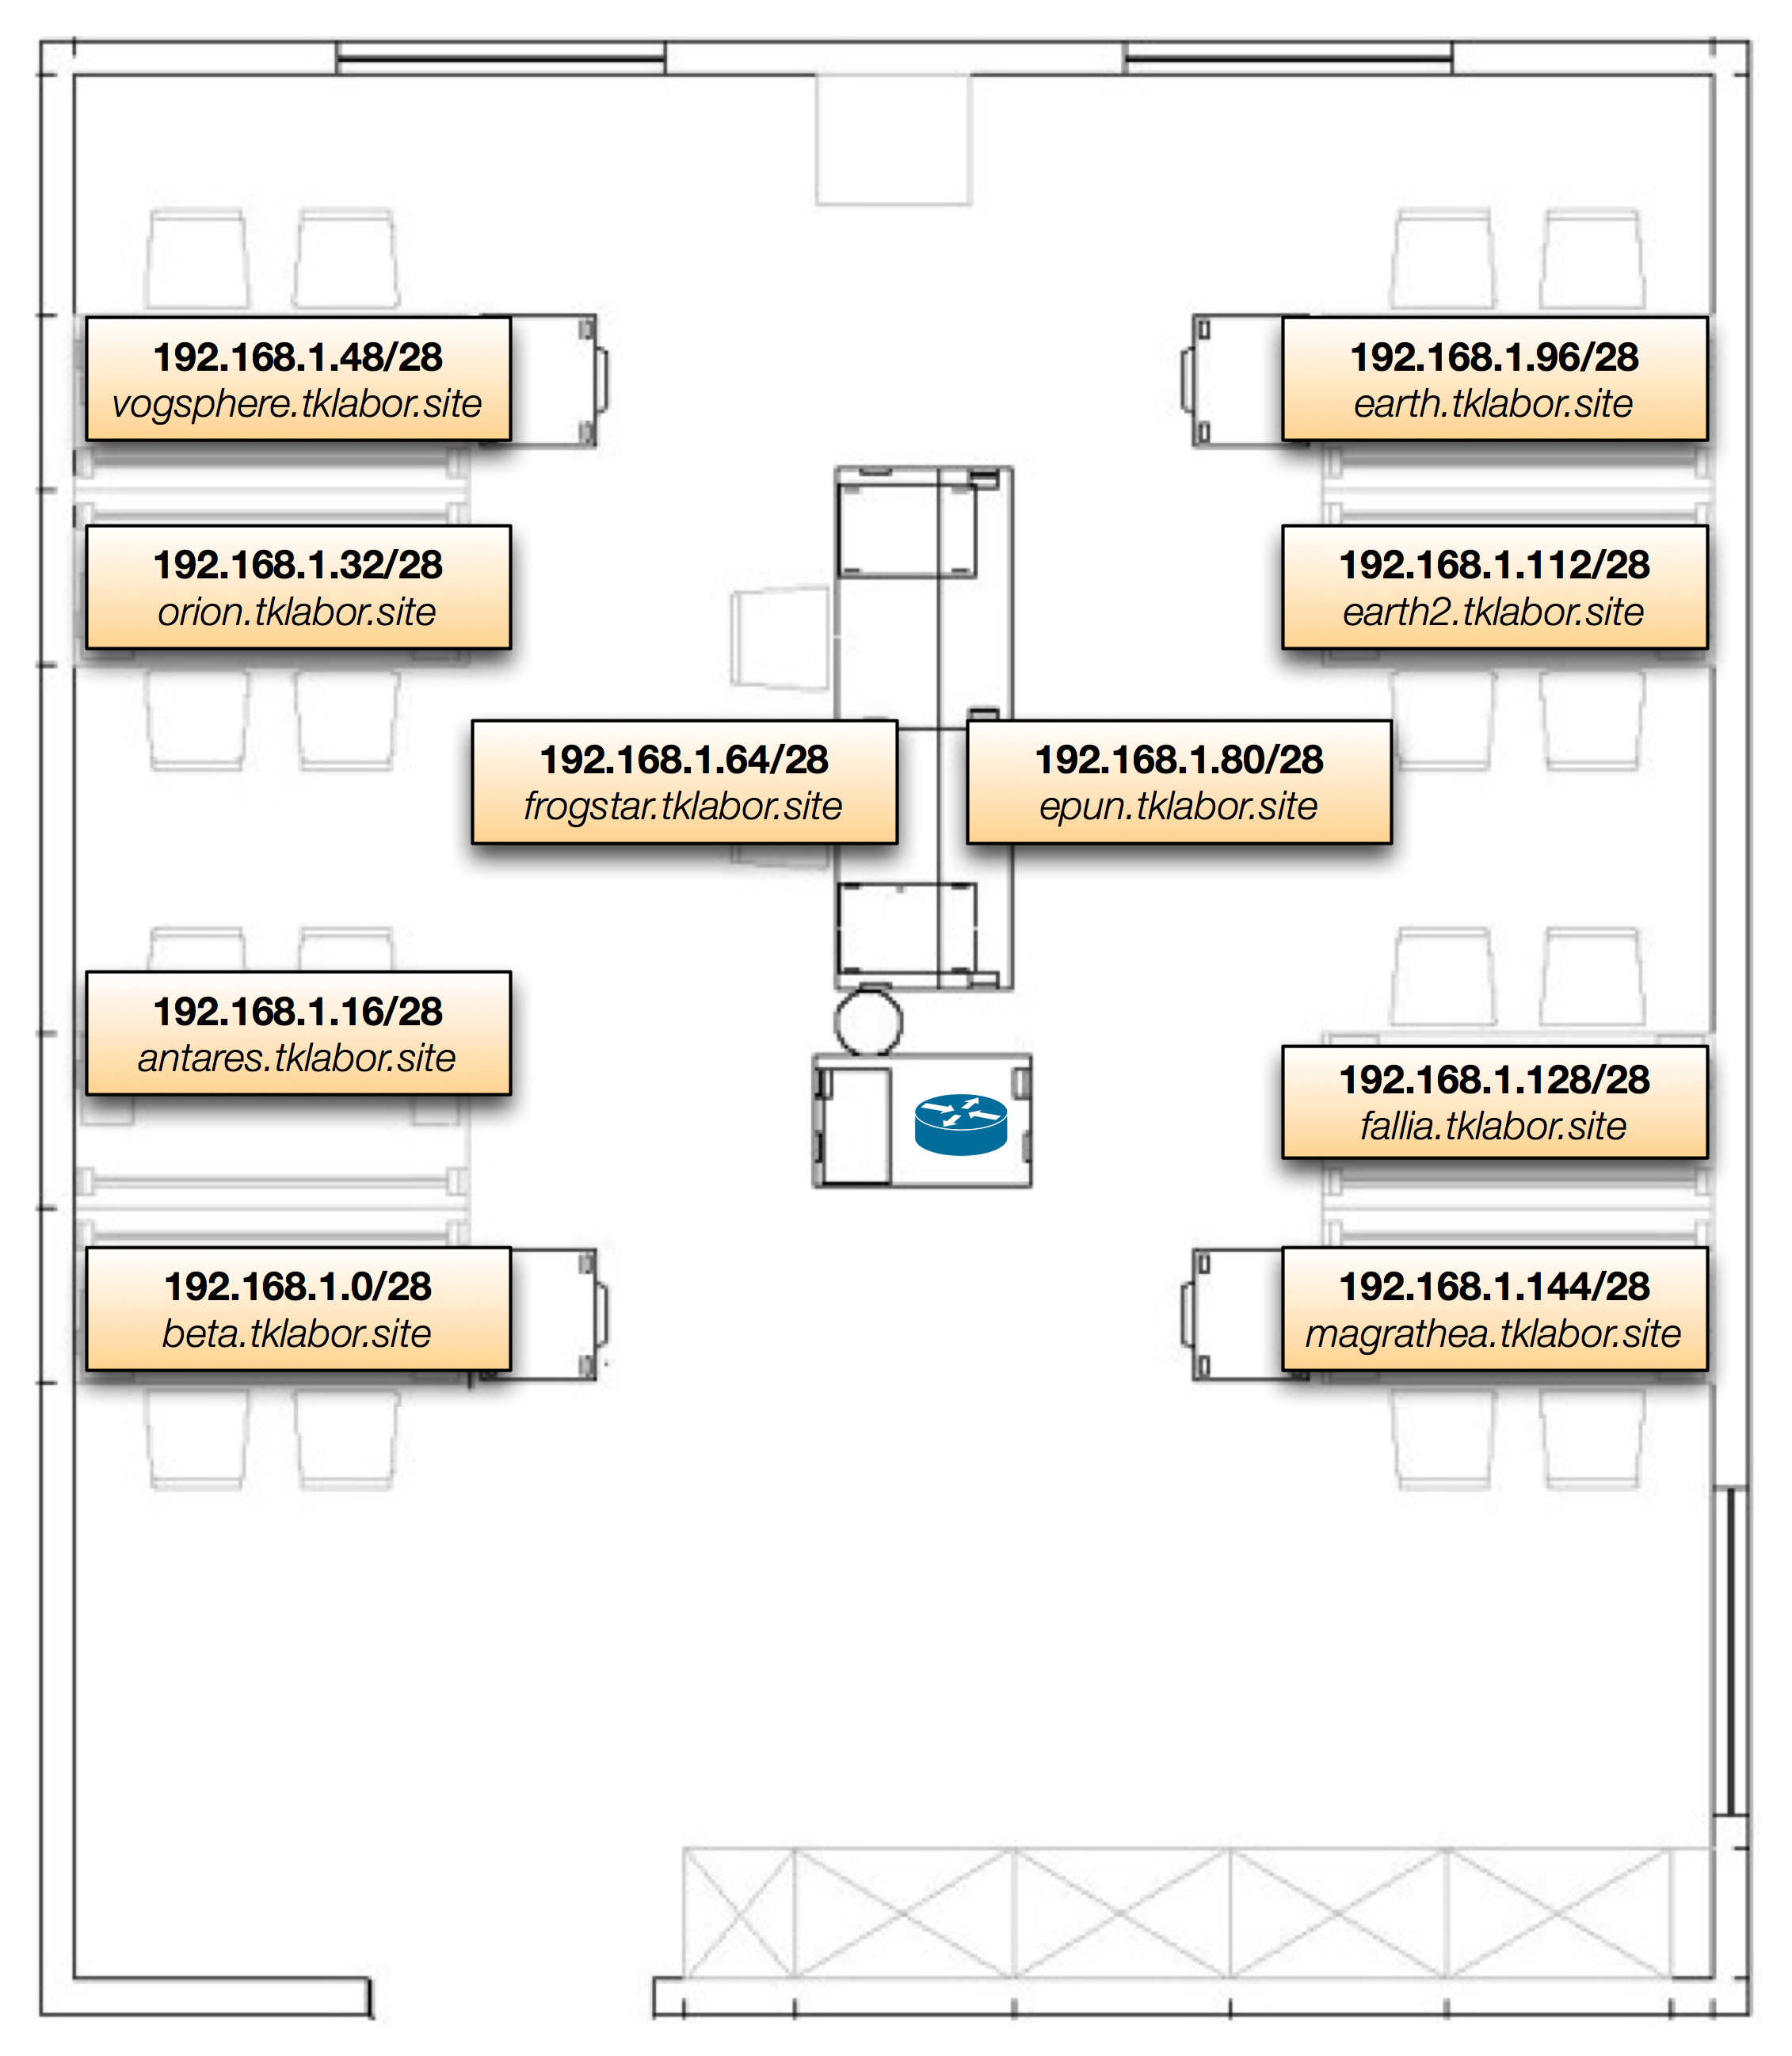
\includegraphics[width=0.75\textwidth]{images/lab-aufbau.png}
\end{center}
\end{figure}

\section{Vorbereitung}
In dieser Übung soll das Zusammenspiel grundlegender Internetdienste veranschaulicht werden.
Hierfür werden zwei virtuelle Maschinen benötigt, die im Folgenden erstellt werden. Dabei sind folgende
Werte entsprechend zu setzen.

\scriptsize\begin{tabular}[t]{l l l l l}
\hline
Name (VMware) & Pfad (VMware) & Hostname & Benutzername & Passwort \\
\hline
srv1-0 & D:$\backslash$Austausch$\backslash$Internetdienste$\backslash$srv1-0 &
srv1-0 & admin1 & password1 \\
srv2-0 & D:$\backslash$Austausch$\backslash$Internetdienste$\backslash$srv2-0 &
srv2-0 & admin2 & password2 \\
\hline
\end{tabular}

\normalsize \subsection{Erzeugung der virtuellen Maschinen}
Im Folgenden wird die Erzeugung einer virtuellen Maschine mit VMware-Workstation exemplarisch für \textbf{srv1} gezeigt. Verfahren Sie für die Maschine \textbf{srv2} analog.
Öffnen Sie das Programm  \textbf{VMware Workstation} und wählen Sie \textbf{File$\rightarrow$New$\rightarrow$Virtual Machine} im Menü.

\begin{figure}[H]
\begin{center}
\includegraphics[width=0.85\textwidth]{screenshots/vm1.png}
\end{center}
\end{figure}

\pagebreak
Im nun erscheinenden Dialog aktivieren Sie die Option \textbf{Typical}. Danach klicken Sie auf \textbf{Next} um zur nächsten Seite des Assistenten
zu gelangen.

\begin{figure}[H]
\begin{center}
\includegraphics[width=0.85\textwidth]{screenshots/vm2.png}
\end{center}
\end{figure}

Hier muss die Option \textbf{I will install the operation system later} gewählt werden. Wieder geht es mit einem
Klick auf \textbf{Next} zur nächsten Seite.

\begin{figure}[H]
\begin{center}
\includegraphics[width=0.85\textwidth]{screenshots/vm4.png}
\end{center}
\end{figure}

\pagebreak
Wählen Sie nun als Betriebssystem \textbf{Linux} und als Version \textbf{Ubuntu} und bestätigen Sie diese
Eingaben mit einem Klick auf \textbf{Next}.

\begin{figure}[H]
\begin{center}
\includegraphics[width=0.85\textwidth]{screenshots/vm5.png}
\end{center}
\end{figure}

Geben Sie nun den Namen \textbf{srv1} und als Speicherort den Pfad \\ \textbf{D:$\backslash$Austausch$\backslash$Internetdienste$\backslash$srv1} an.

\begin{figure}[H]
\begin{center}
\includegraphics[width=0.85\textwidth]{screenshots/vm6.png}
\end{center}
\end{figure}

\pagebreak
Für die Größe der virtuellen Festplatte wählen Sie bitte \textbf{8} Gigabyte.

\begin{figure}[H]
\begin{center}
\includegraphics[width=0.85\textwidth]{screenshots/vm7.png}
\end{center}
\end{figure}

Der folgende Dialog wird jetzt mit \textbf{Finish} geschlossen.

\begin{figure}[H]
\begin{center}
\includegraphics[width=0.85\textwidth]{screenshots/vm8.png}
\end{center}
\end{figure}

\pagebreak
Als nächsten müssen noch einige Einstellungen der virtuellen Maschine bearbeitet werden. Hierzu wählen Sie
\textbf{Edit virtual machine settings}.

\begin{figure}[H]
\begin{center}
\includegraphics[width=0.85\textwidth]{screenshots/vm9.png}
\end{center}
\end{figure}
Wählen Sie nun den Eintrag \textbf{CD/DVD} und aktivieren Sie die Option \textbf{Use ISO image file}. Klicken Sie auf \textbf{Browse}
und wählen Sie die Datei \\ \textbf{D:$\backslash$Austausch$\backslash$Internetdienste$\backslash$ubuntu-10.10-server-i386.iso}.

\begin{figure}[H]
\begin{center}
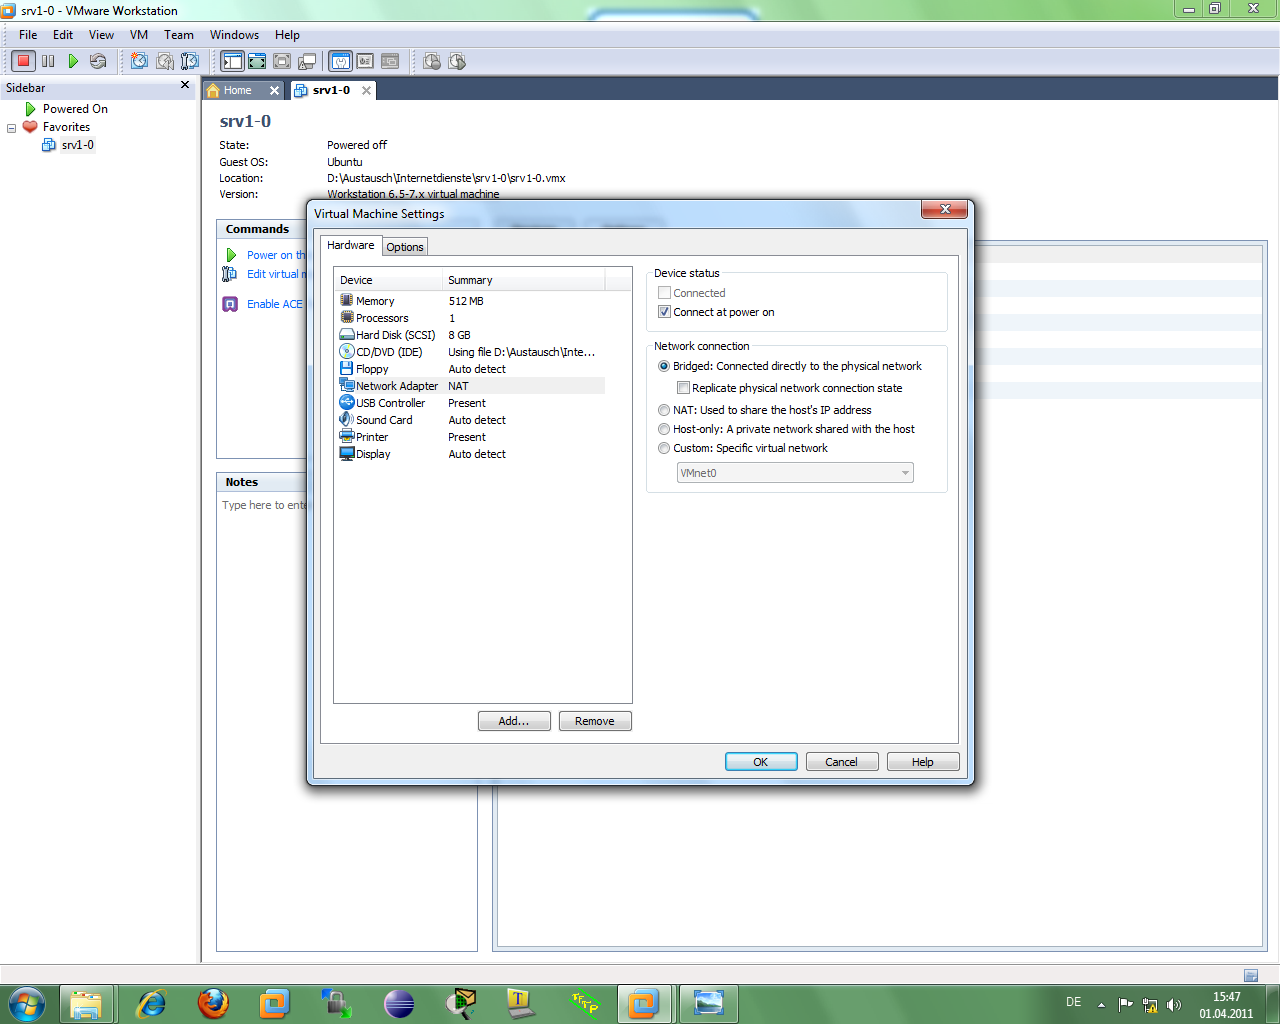
\includegraphics[width=0.85\textwidth]{screenshots/vm10.png}
\end{center}
\end{figure}

\pagebreak
Danach wählen Sie den Eintrag \textbf{Network adapter} und aktivieren die Option \textbf{Bridged}.

\begin{figure}[H]
\begin{center}
\includegraphics[width=0.85\textwidth]{screenshots/vm11.png}
\end{center}
\end{figure}

Verfahren Sie analog für den Server \textbf{srv2}.

\end{document}
